\providecommand{\main}{../../../..}
\documentclass[\main/dresen_thesis.tex]{subfiles}

\begin{document}
  As the dispersion is composed of a fast and slow evaporating component, the drop casting process subdivides into two parts.
  The first, where the primary fast evaporating phase of the dispersion evaporates and the second where the slowly evaporating phase is removed.
  For the first part, different conditions can be tested: it can be performed on a heating or cooling stage to change the surface temperature of the wafer, a magnetic field can be applied or the drying time can be enlarged by performing the drying procedure within an enclosed container.
  Reducing the wafer temperature by the means of a Peltier element is, however, not improving the structure as the 1-octadecene quickly freezes the dispersion at temperatures around $16 \unit{^\circ C}$.
  Applying an in-plane magnetic field to strongly magnetic nanocubes during the first drying stages by the means of an Halbach ring shows qualitatively a tendency of aligning the cubes with the (100) faces along the magnetic field, as well as an improvement of the general structure as visible from SEM shown in \reffig{fig:monolayers:preparation:dryingConditions:magneticField}.
  \begin{figure}[tb]
    \centering
    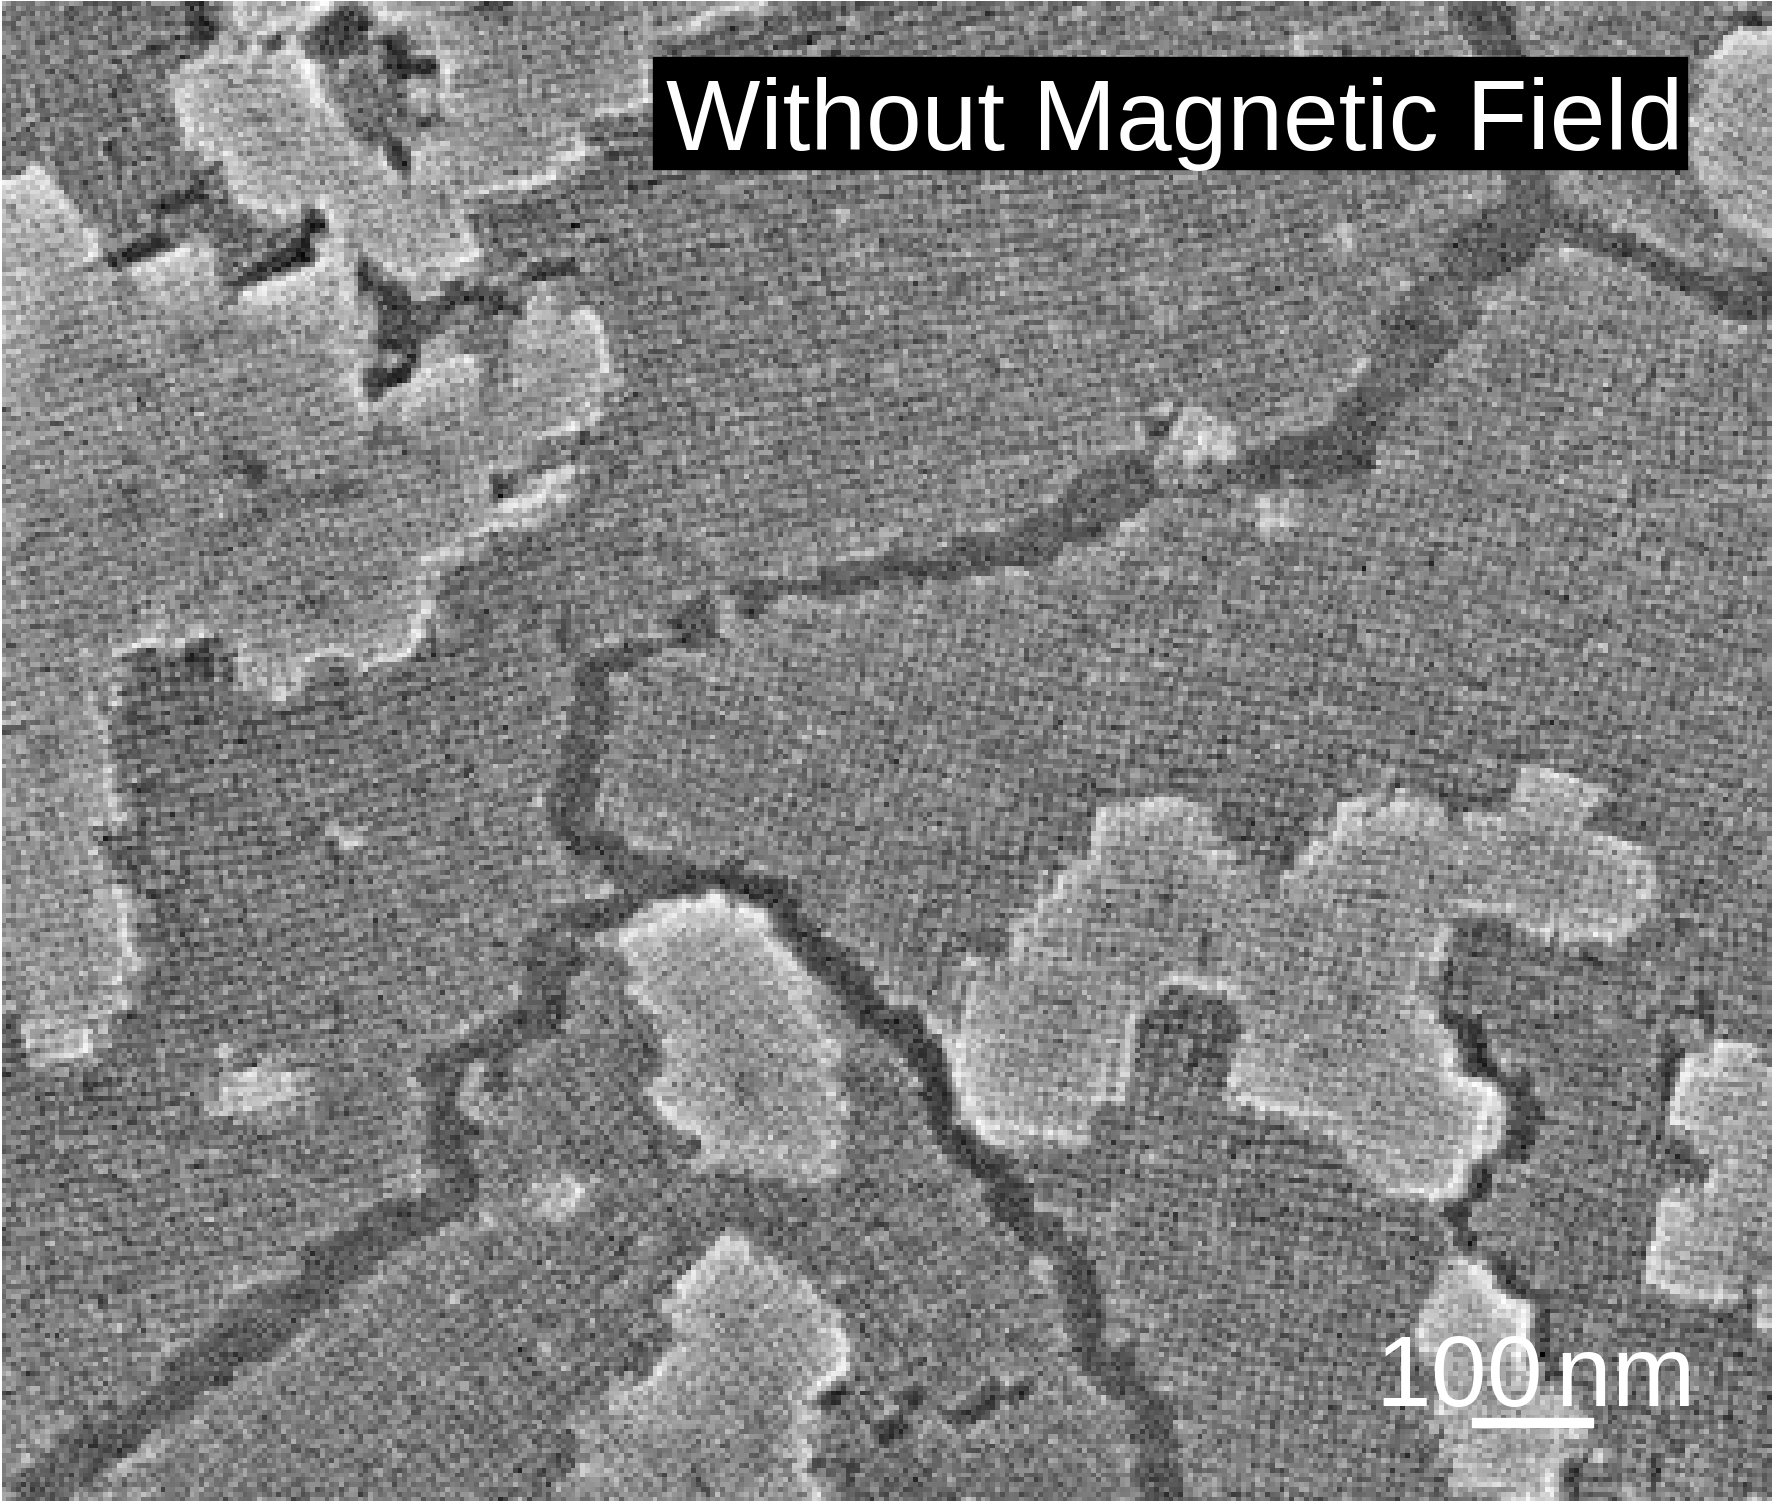
\includegraphics{monolayers_SEM_without_mag_field}
    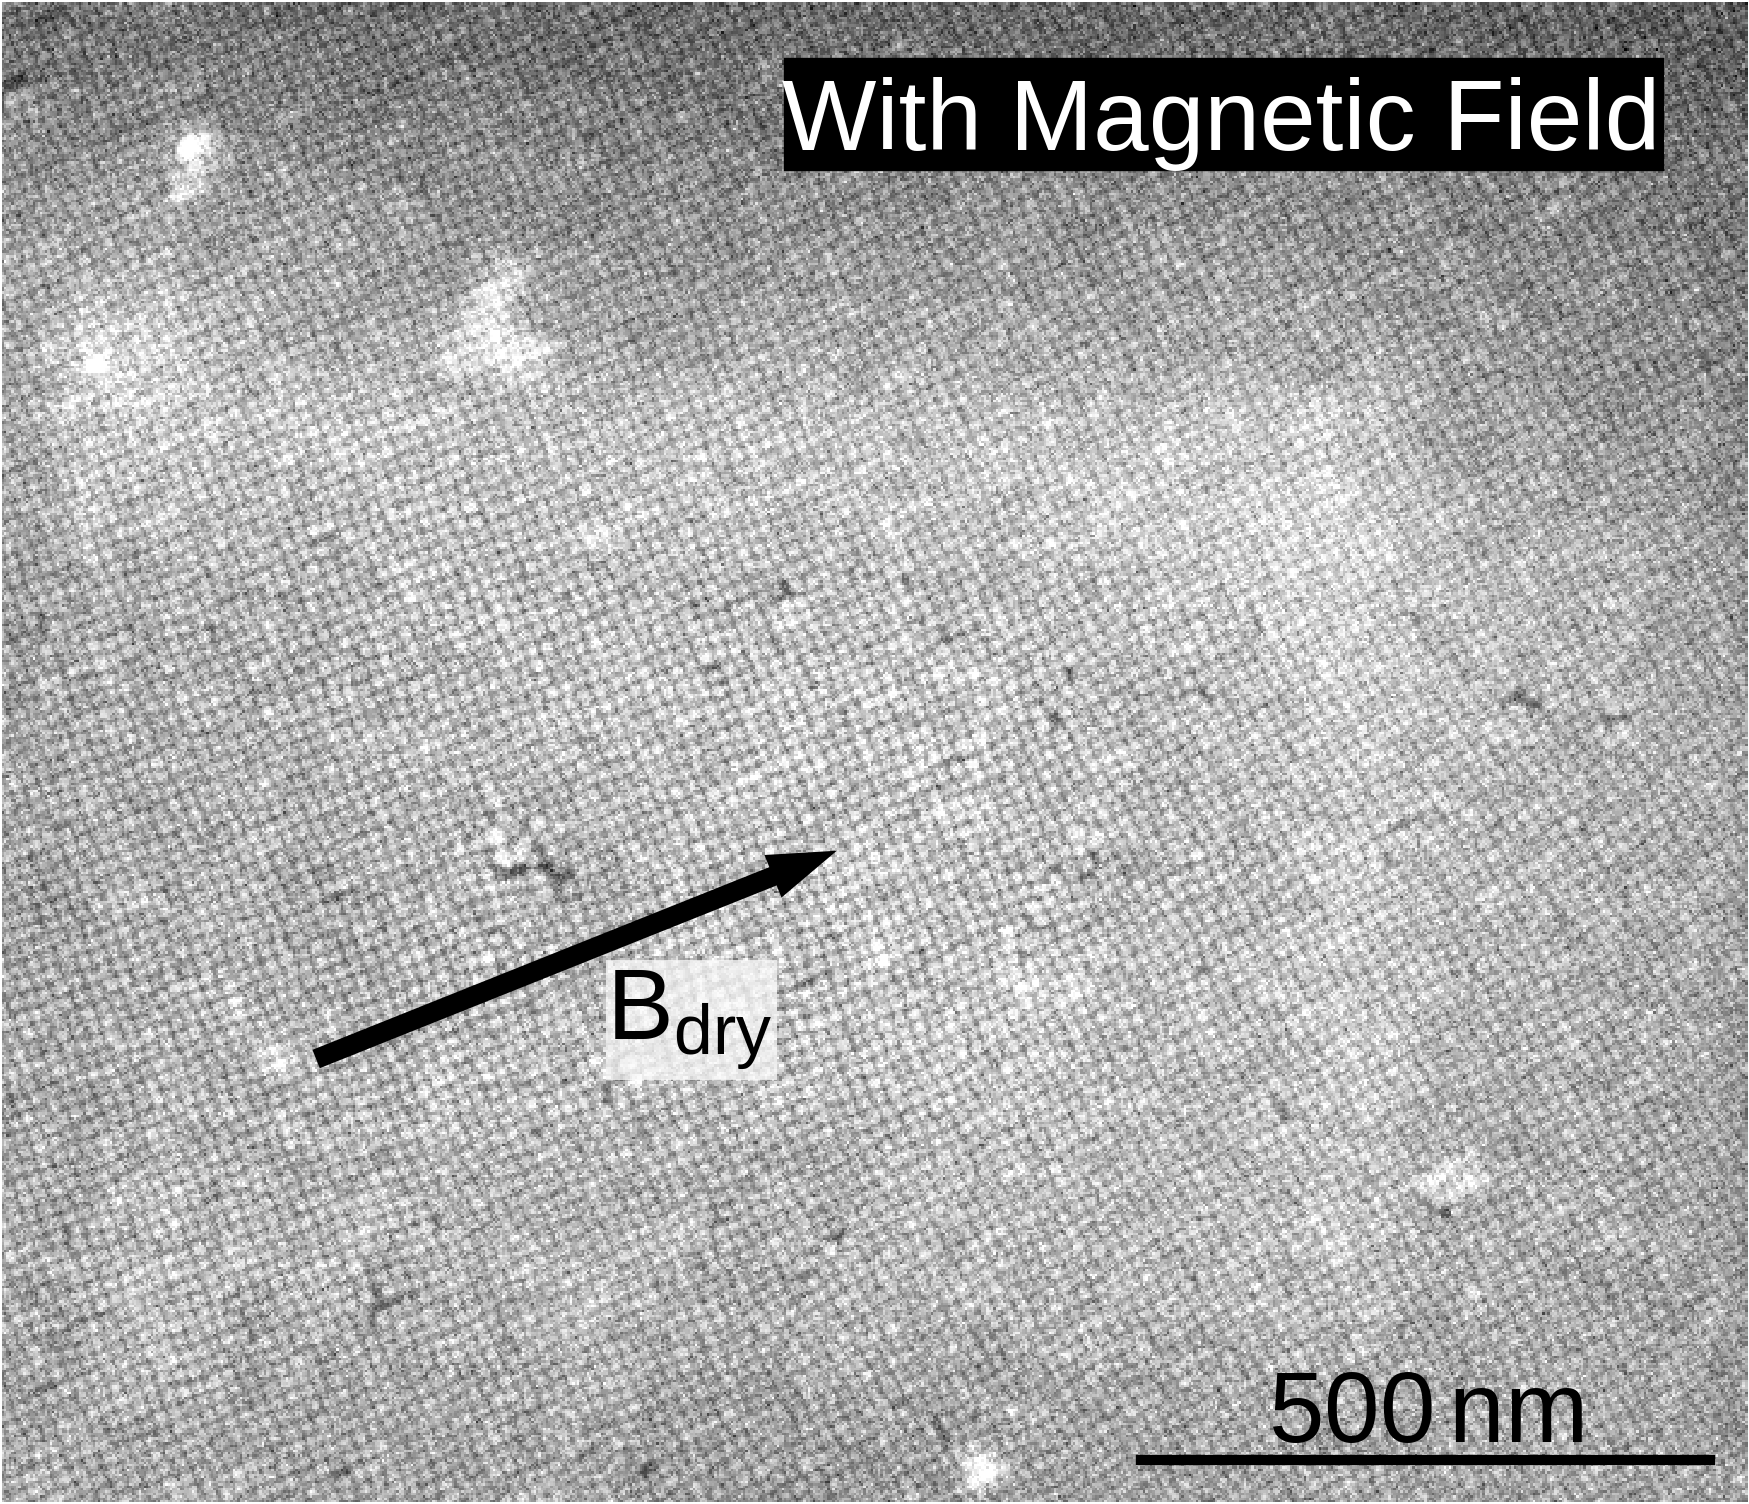
\includegraphics{monolayers_SEM_with_mag_field}
    \caption{\label{fig:monolayers:preparation:dryingConditions:magneticField}Comparison of simultaneously prepared monolayer from the same dispersion, one without applying a magnetic field, one within a Halbach ring with $B_{dry} \eq 40 \unit{mT}$.}
  \end{figure}
  A detailed quantitative study of these structures is, however, not part of this work.
  For all presented samples the first evaporation step is always performed at ambient conditions, in an open container, on an even surface, within a calm room as this has shown to provide the best results in all initial tests.

  \begin{figure}[tb]
    \centering
    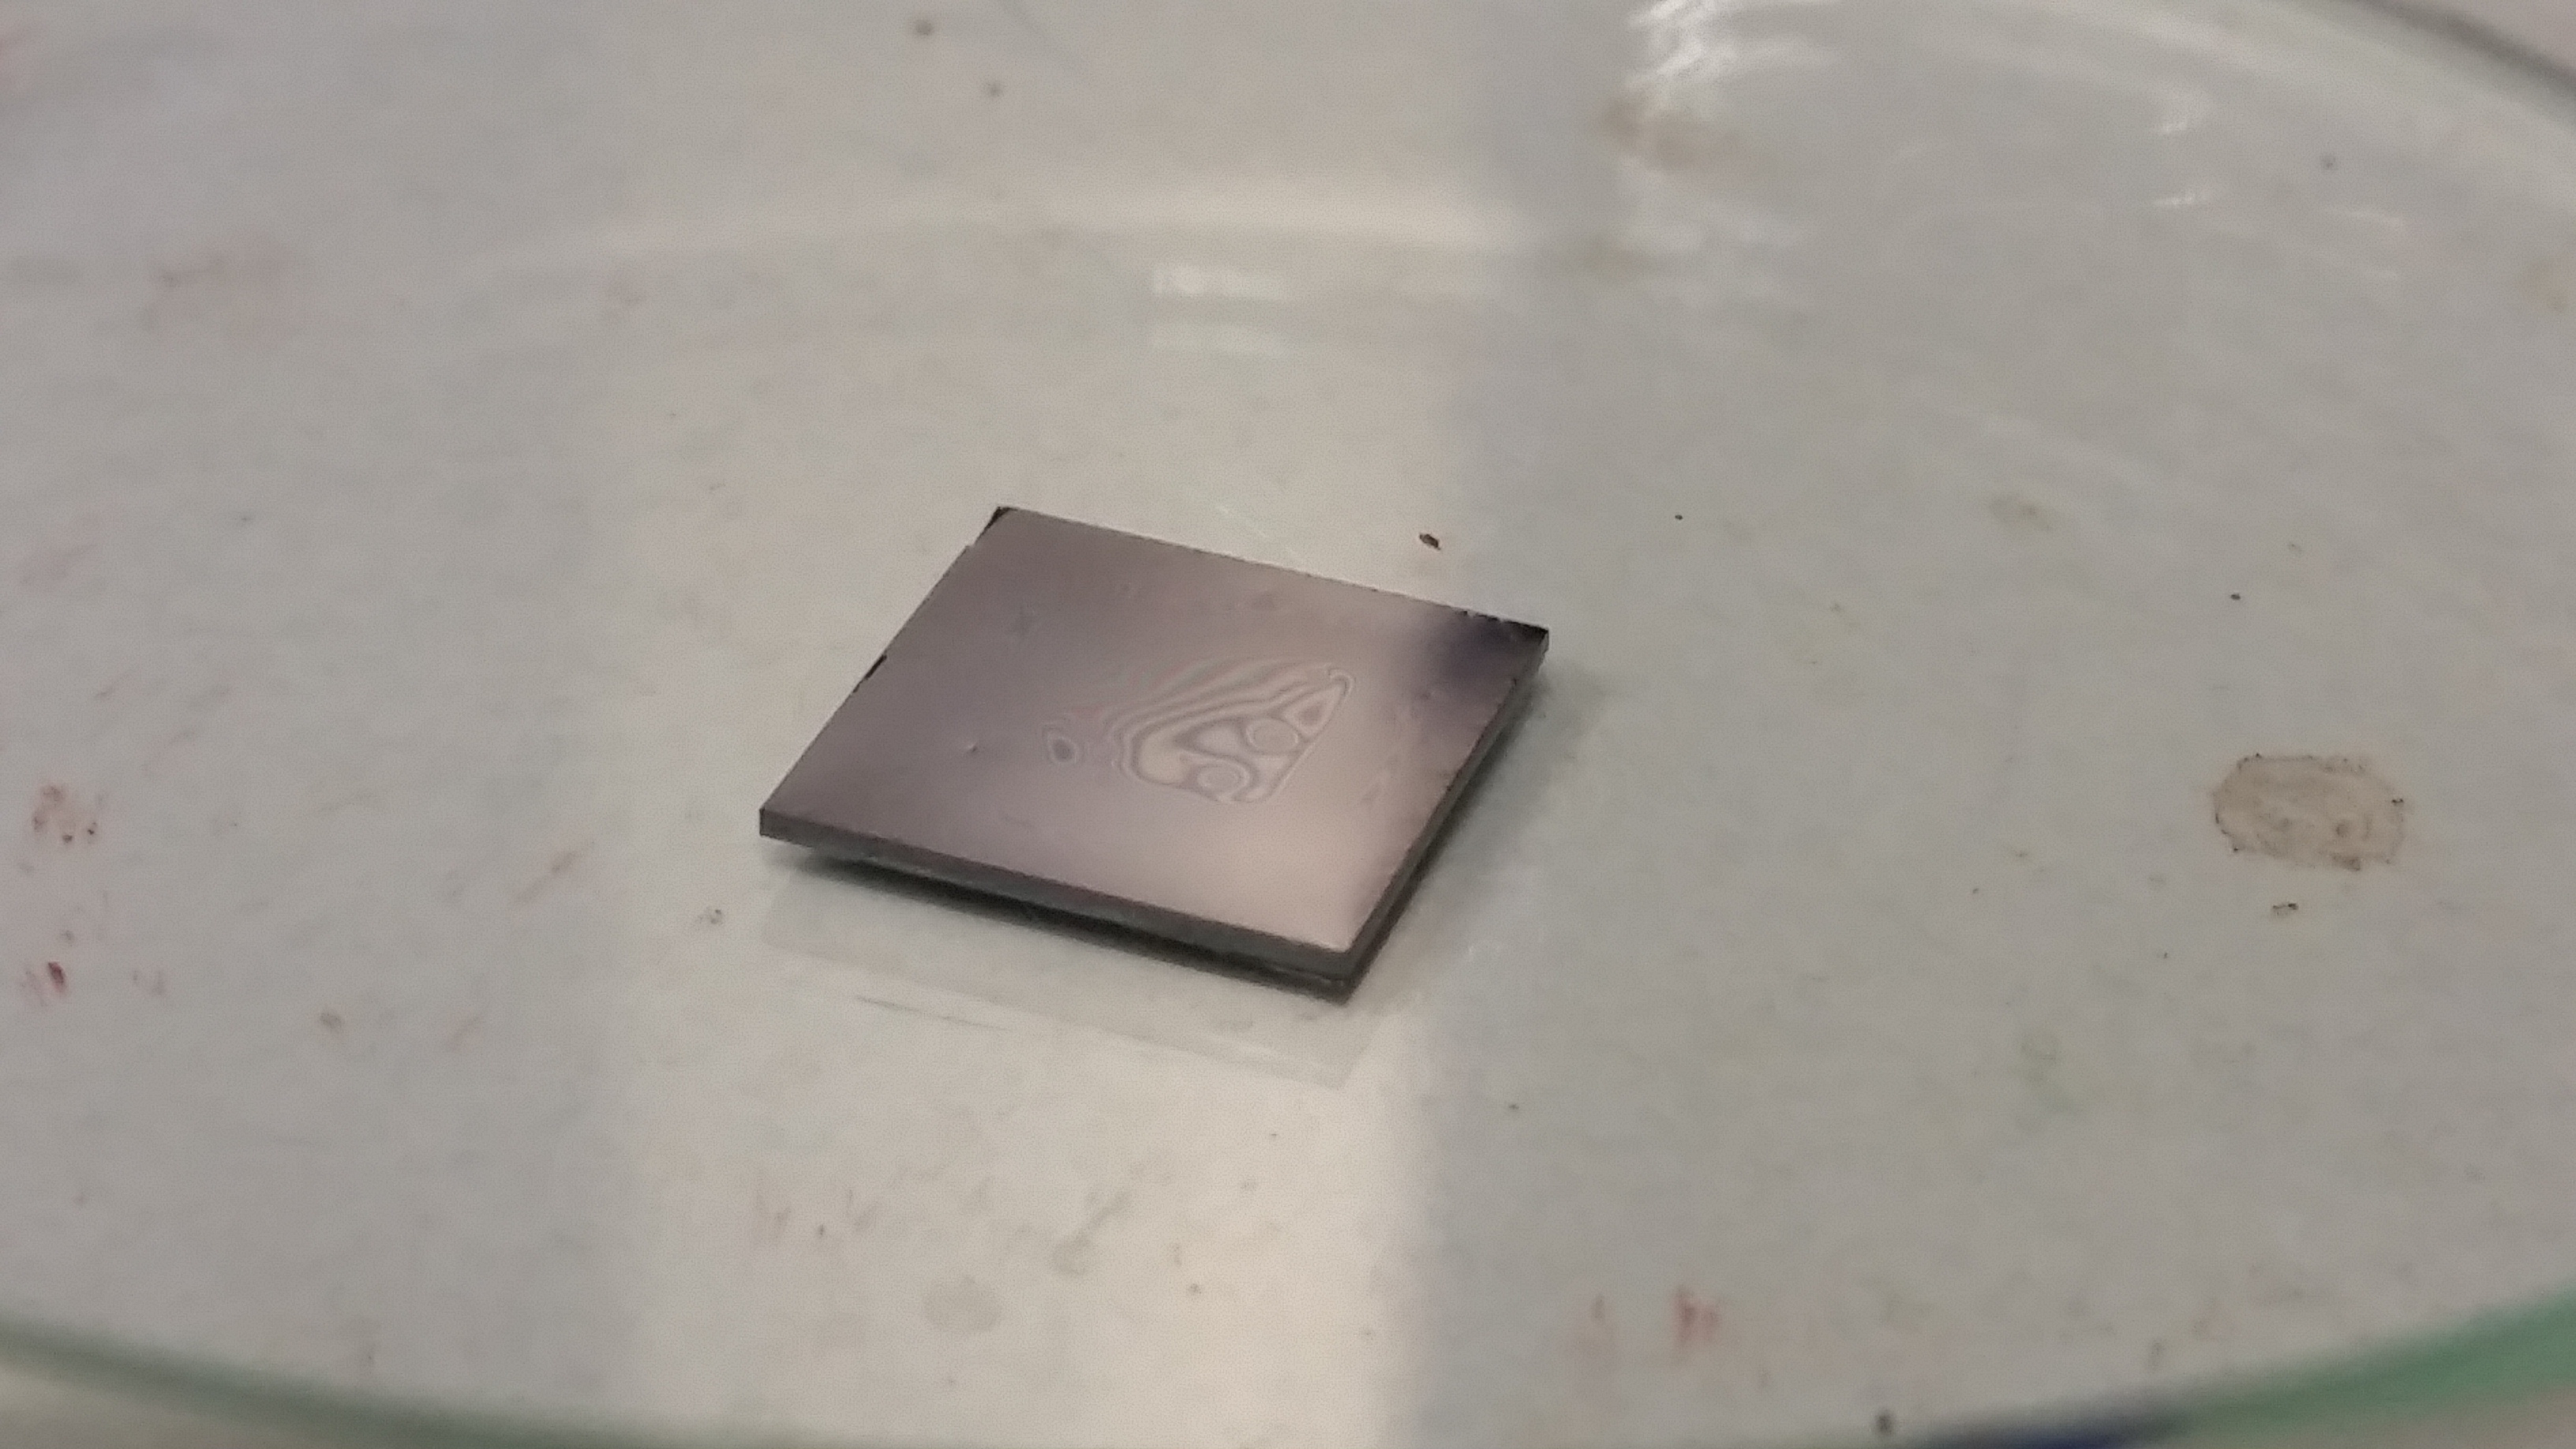
\includegraphics[width=0.7\textwidth]{monolayers_preparation_oilyFilm}
    \caption{\label{fig:monolayers:preparation:dryingConditions:oilyFilm}Thin oily film visible on a silicon wafer after the fast evaporating component of the dispersion has been dried during monolayer preparation.}
  \end{figure}
  After the fast evaporating component of the dispersion is dry, a thin oily film is visible on the wafer by thin-film interference as shown in \reffig{fig:monolayers:preparation:dryingConditions:oilyFilm}.
  Even after several weeks, the thin-film of 1-octadecene/oleic acid does not evaporate at room temperature and has to be removed actively at elevated temperatures.
  While temperatures of at least $140 \unit{^\circ C}$ are necessary to remove the organic components to most parts, quickly heating to that temperature (via a heating plate for example) leads to a inhomogeneous evaporation of the droplet.
  To have a homogeneous evaporation, the best found method is to place the silicon wafer within a glass Petri dish that is covered with perforated aluminium foil.
  Then, the best result is observed when the thin film is left within an oven at $80 \unit{^\circ C}$ for at least $12\unit{h}$ and only then heated to $140 \unit{^\circ C}$ for at least $6\unit{h}$.
  It is important to balance the oven with a water level, as any slope leads to a accumulation at the lower side of the silicon wafer.
\end{document}